\documentclass[12pt]{article}

\title{The limits of parallelism in adaptation due to domestication in the grasses}
\author{Woodhouse, M.R. and M. B. Hufford}

\usepackage[utf8]{inputenc}
\usepackage{colortbl}
\usepackage[letterpaper, margin=1in]{geometry} %package that allows changes in margins and header/footers
\usepackage{authblk}%allows footnote format for authors
\usepackage{rotating}
\usepackage{amsmath}
\usepackage{array}
\usepackage{booktabs}
\usepackage[x11names,dvipsnames,table]{xcolor}
\usepackage{tabularx}
\usepackage{mathptmx}       % selects Times Roman as basic font
\usepackage{helvet}         % selects Helvetica as sans-serif font
\usepackage{courier}        % selects Courier as typewriter font
\usepackage{type1cm}        % activate if the above 3 fonts are
                            % not available on your system
%
\usepackage{natbib}
\usepackage{makeidx}         % allows index generation
\usepackage{graphicx}        % standard LaTeX graphics tool
                             % when including figure files
\usepackage{multicol}        % used for the two-column index
\usepackage[bottom]{footmisc}% places footnotes at page bottom
\usepackage{setspace}
\usepackage{gensymb}
\usepackage{color}
\usepackage[textsize=tiny,colorinlistoftodos]{todonotes} % comments in margins

\definecolor{cornflowerblue}{rgb}{0.39, 0.58, 0.93}
\newcolumntype{G}[1]{>{\raggedright\let\newline\\\arraybackslash\hspace{0pt}}m{#1}}
\newcolumntype{C}[1]{>{\centering\let\newline\\\arraybackslash\hspace{0pt}}m{#1}}
\newcommand{\mbh}[1]{\textcolor{red}{\normalsize  #1}}
\newcommand{\mw}[1]{\textcolor{cornflowerblue}{\normalsize #1}}

\begin{document}
\maketitle

\begin{abstract}
The selection of desirable traits in crops during domestication has been well studied.
Many crops share a suite of phenotypic characteristics collectively known as the domestication syndrome.
Previous work has demonstrated that, at least in some instances, parallel selection of orthologous loci across species has resulted in shared domestication traits.
However, both demography and selection during domestication can place limits on the evolutionary potential for subsequent adaptation and reduce opportunities for parallelism.
Here we review current knowledge regarding the extent of parallelism versus convergence during domestication and adaptation in the grasses and consider whether the dynamism of grass genomes (e.g., transposable elements, polyploidy, genome size), help these species overcome their legacy of domestication to achieve broad subsequent adaptation.
\end{abstract}

\section*{Introduction}
Human societies rely heavily on domesticated crop species for survival.
For example, considering crop production as a measure of consumption, in 2016 alone the United States produced 384 million tons of maize, China produced 211 million tons of rice, and Nigeria produced 6.9 million tons of sorghum \citep{FAOSTAT2018}.
Human reliance on crops has deepened over the last $\approx10,000$ years, as crops have been continually selected by humans for traits including nutrition, yield, and other attractive features, a process that has also dramatically changed crop physiology.
As such, domesticated crops are often radically different from their wild relatives.
Notably, there are several traits beyond yield and nutrition that often distinguish domesticated crops from their wild progenitors \citep{Doebley2006}, distinctions that are frequently shared even among distantly related crops such as maize and sunflower.
These traits include apical dominance or lack of branching, loss of seed dormancy, loss of bitterness, and loss of shattering or seed dispersal (Table \ref{tab:DomTraits}).
This suite of shared traits is collectively known as the domestication syndrome \citep{Hammer1984}.

\begin{table}
\rowcolors{2}{gray!25}{white}
\begin{center}
\caption{Prevalence of Domestication Syndrome Traits} \label{tab:DomTraits}
\begin{tabular}{p{5cm}cccl}\\\toprule  
{\bf Domestication Trait} & {\bf In Grass Crops} & {\bf In non-Grass Crops} &	{\bf References} \\\toprule
Compact plant growth & yes & yes & \citep{Gepts2010, Lenser2013}\\
Reduced axillary branching & yes & yes & \citep{Lenser2013}\\
Reduced seed dormancy & yes & yes & \citep{Gepts2010, FernndezMarn2014}\\
Changes in flowering time & yes & yes & \citep{Lenser2013}\\
Uniform flowering or maturation time & yes & yes & \citep{Lenser2013}\\
Vernalization & yes & yes & \citep{Blackman2016}\\
Increased resource allocation to harvested organ/larger organ (fruit, grain, root) & yes & yes & \citep{Miller2011}\\
Compact inforescence & yes & yes & \citep{Gepts2010, Greenwood2017}\\
Non-shattering/indehiscent fruit or grain & yes & yes & \citep{Lenser2013, Dong2014}\\
Changes in pigmentation & yes & yes & \citep{Lenser2013}\\
Self-fertilizing & yes & yes & \citep{Gepts2010}\\
Perennial to annual lifecycle  & yes & yes & \citep{Gepts2010, Miller2011}\\
Sexual to vegetative reproduction & no & yes & \citep{Lyu2017}\\
Reduced defensive structures (spines, thorns) & no & yes & \citep{Miller2011, Pickersgill2007}\\
Reduced toxicity & no & yes & \citep{Miller2011, Shlichta2018}\\
Soft or naked kernel or seed & yes & no & \citep{Wang2005}\\
Increased spikelets & yes & no & \citep{Gepts2010}\\
Increased number of kernel rows & yes & no & \citep{Lenser2013}\\\bottomrule
\end{tabular}
\end{center}
\end{table} 
 

But how can two vastly diverged species such as maize and sunflower  (their last common ancestor was 150 MYA \citep{Chang2004}) share the same domestication traits? 
Since these two species still share enzymatic pathways, perhaps orthologous genes or genes with similar physiological roles have been targeted by selection during domestication.
Shared phenotypes caused by repeated modification of orthologs, is a phenomenon known as parallelism; parallelism is more likely to occur in closely related species due to their similar complement of genes \citep{Pickersgill2018}.
Conversely, it is possible for unrelated genes in different enzymatic pathways to give rise to similar traits, particularly when species experience similar selection pressures (either human or environmental), such as fruit/seed indehiscence in both dicot and monocot crops (reviewed in \citep{Dong2015}).
This phenomenon, known as convergence, is more likely to occur in substantially diverged species that contain fewer orthologous loci and pathways \citep{Washburn2016, Pickersgill2018}.

After the initial wave of crop domestication yielded many of the aforementioned domestication syndrome traits, another level of differentiation ensued--the adaptation of crop species to varied environmental conditions during global expansion.
A cultivar of maize bred for cultivation at sea level, for instance, may not necessarily thrive in the colder, higher UV environment of the Andes.
Therefore, cultivators in the Andes must have looked for individuals in the existing domesticated maize population that were hardy under these new conditions.
However, crop adaptation faced genetic limitations not experienced during domestication of wild progenitors \cite{Wang2017}. 

Only a subset of genome-wide diversity was retained in initial domesticates and additional diversity was lost through subsampling events during crop expansion.
Furthermore, selection on particular alleles coding for desirable traits (such as those comprising the domestication syndrome) often resulted in dramatic reductions in diversity in particular chromosomal regions.
The effects of this loss of genetic diversity on the potential for adaptation has been documented.
For example, a dramatic genetic bottleneck in the ``lumper" variety of potato led to a catastrophic outbreak of \emph{Phytopthera infestans}, resulting in the infamous Potato Famine in Ireland in the 1840s \citep{Goodwin1994}.
The Potato Famine demonstrated that by divesting a crop cultivar of its diversity, the cultivar also loses its ability to adapt to newly encountered environmental pressures, because the alleles that code for adaptive traits such as, for instance, disease resistance are lost.

This review will focus on the extent of parallelism and convergence in both crop domestication and adaptation and consider the extent to which early bottlenecks have affected the potential for parallelism and convergence during post-domestication adaptation.
We will focus mainly on grass crops, since the major domesticates--maize, rice, sorghum, wheat, barley, and millet--include a range of divergence times conducive to adaptation and evolution of domestication syndrome traits through both parallelism and convergence.
Grasses also share a certain amount of genomic dynamism, including polyploidization and transposable element activity, that provides diversity upon which selection can act.
We examine the relationship between domestication and adaptive traits, how domestication bottlenecks reduce population diversity, and look at the ways in which the dynamic nature of grass genomes might potentially increase genomic diversity to facilitate adaptation despite bottlenecks during domestication and expansion.
\paragraph{}

\section*{Domestication in the grasses}
Grasses have often been studied as a cohesive genetic group \citep{pmid8379002, pmid11244100}, and there are many reasons why they present a compelling system for studying crop domestication.
The grass clade is thought to have arisen around 75 MYA \citep{BOUCHENAKKHELLADI2010, Kellogg2001} with rice, wheat, barley, millet, maize, and sorghum arising sequentially afterward (Figure \ref{fig:grassphylo}).
Prior to the radiation of the grasses, however, a genome duplication event occurred approximately 70 MYA \citep{Paterson2004}, which is shared among all grass crops (Figure \ref{fig:grassphylo}).
Subsequently, both maize and wheat have undergone additional, lineage-specific polyploidy events (Figure \ref{fig:grassphylo}) \citep{Levy2002}.
These polyploidy events, followed by selective and ongoing fractionation, present an opportunity for grass genomes to evolve subfunctionalized homeologs; this, along with relatively high transposon activity (particularly in maize and wheat) that can give rise to functional mutation \citep{Wicker2016, Lisch2001}, make the grasses a useful system for studying the potential for adaptation after a domestication bottleneck.

Additionally, most grass crops were domesticated within the latitudinal boundaries of the equator and 35 N \citep{Jain1993, Gepts2010}, featuring both wet and dry seasons \citep{Jain1993}, which means that many domesticated grasses shared similar environmental pressures such as temperature, precipitation and day length.
However, each grass cereal has been cultivated in separate geographic locations, including maize (Americas), sorghum (Africa), rice (Asia), millet (Eurasia), and wheat and barley (the Middle East) \citep{Glmin2009}, and, to some extent, approaches to domestication in these separate regions were guided by culturally distinct selection of traits.
Taken together, these features make domesticated grass species especially conducive to the meaningful study of convergence and parallelism.


\begin{figure}[h]
    \centering
    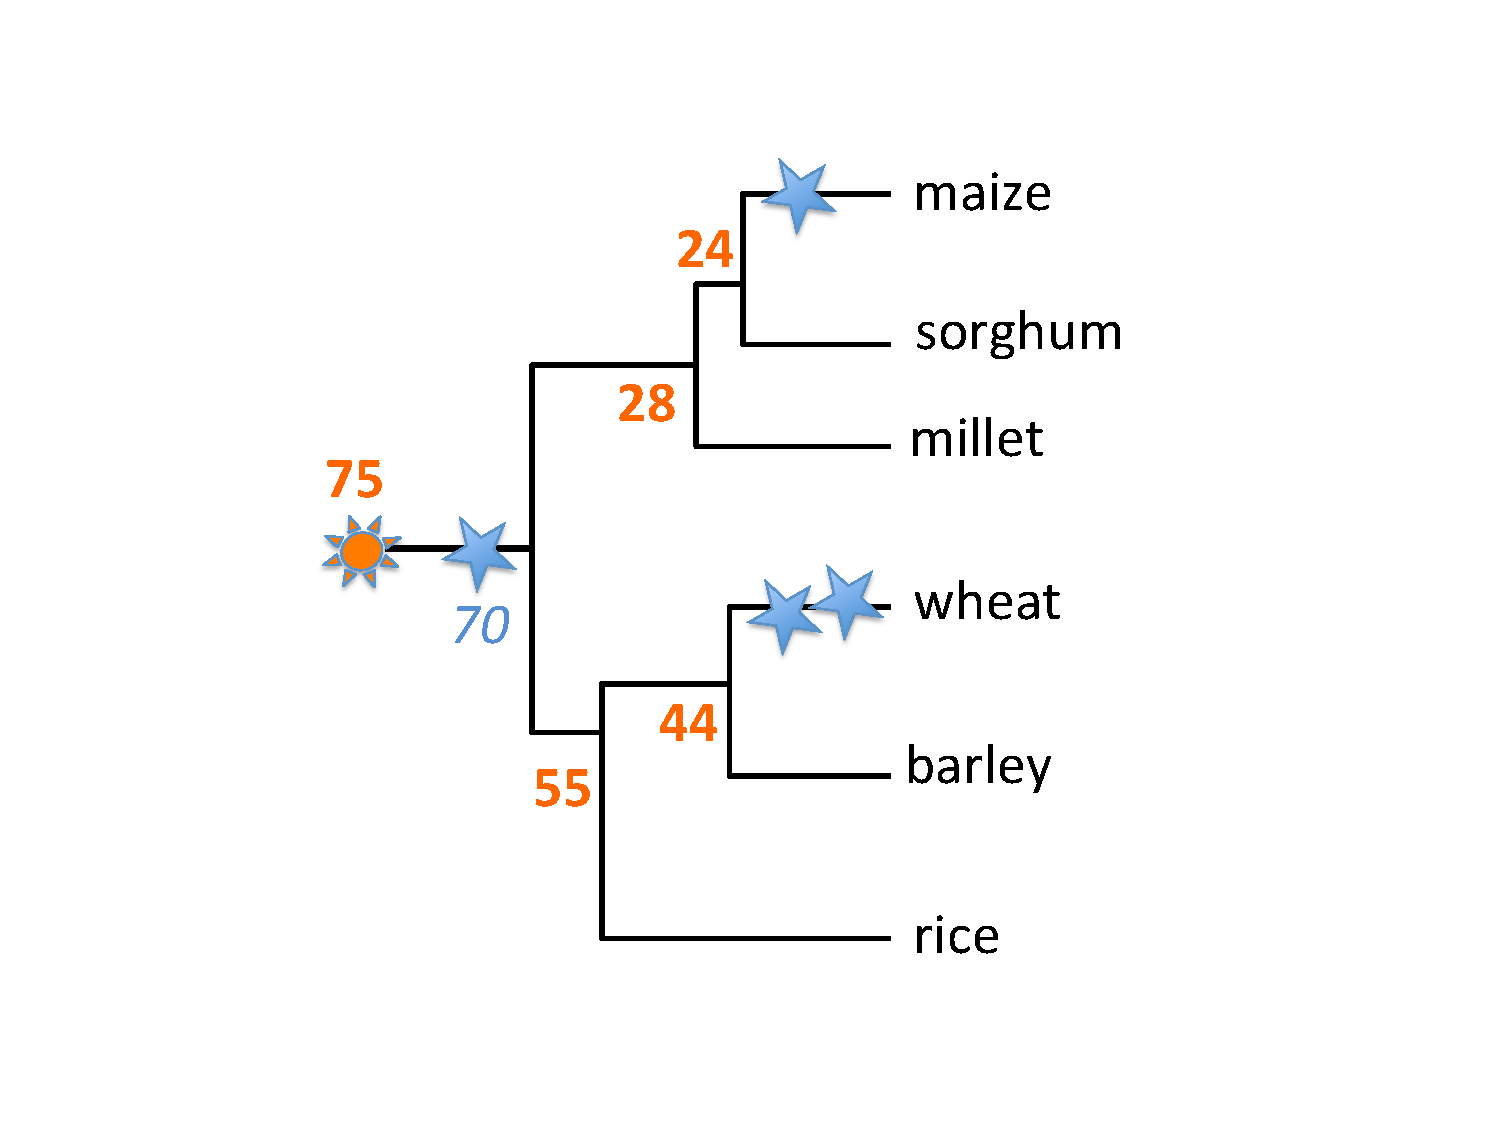
\includegraphics[width=15cm]{Figure_1.pdf}
    \caption{Simple cladogram of major cereal speciation. Numbers are in MYA (millions of years ago).
Orange sun: grass speciation event 75 MYA.  Blue stars: polyploidy events; 
the major grass polyploidy event immediately after the grass speciation event occurred 
approximately 70 MYA. The Ehrhartoideae clade, which includes rice, arose 
approximately 55MYA. The Pooideae clade, which includes wheat and barley, 
arose around 44MYA; Chloridoideae which contains foxtail millet 28 MYA, and the Panicoids, 
which include maize and sorghum, arose approximately 24MYA. The branch length is not 
proportional to the number of substitutions per site.
}
    \label{fig:grassphylo}
\end{figure}

Grass crops share a number of domestication syndrome traits also observed in non-grass crop species (Table \ref{tab:DomTraits}).
However, some common domestication syndrome traits are notably lacking in the grasses, such as reduced toxicity, vegetative reproduction, and reduced defensive structures like spines and thorns--by and large the wild relatives of grass crops lacked these defense mechanisms.
Likewise, some grass domestication syndrome traits are absent in non-grass crops, such as increased spikelet number and increased number of kernel rows, because these traits occur on structures that are not found outside the grasses.  

An ever-increasing number of causal genes for traits in the domestication syndrome are being identified both within and outside of the grasses; these genes are summarized in Table \ref{tab:Ortho} (modified from \citep{Lenser2013}).
Grass domestication genes can be categorized based on whether they occur strictly within a species, share orthologs across the grasses, share orthologs within and outside of the grasses, or share orthologs entirely outside of the grasses (Column 3, Table \ref{tab:Ortho})
This gives us an opportunity to form hypotheses regarding the likelihood of parallelism and convergence for a certain trait based on its known orthology across taxa. 
For example, in column 8 of Table \ref{tab:Ortho} we indicate whether a domestication gene is expected to be convergent or parallel, based on patterns of orthology.
If a domestication gene is found only within a single species, it obviously cannot be selected in parallel.
For instance, coloration in rice through selection on the \textit{Bh4} gene may be expected to be convergent since this gene's influence on coloration appears to be specific to the rice species.
On the other hand, the coloration gene \textit{BADH2} is found in both rice and soybean, (Table 2), suggesting an example of parallel selection.

\begin{sidewaystable}
\rowcolors{2}{gray!25}{white}
\begin{center}
\caption{Parallel or Convergent Orthologies} \label{tab:Ortho}
        \fontsize{7}{8}\selectfont 
    \begin{tabular}{G{3.5cm}G{2.5cm}C{3.10cm}C{3.5cm}C{1.95cm}G{2.0cm}G{1.8cm}G{1.5cm}G{1.5cm}}
\\\toprule  
{\bf Crop species} & {\bf Ortholog phylogeny} & {\bf Phylogeny of domestication trait} & {\bf Orthologous gene(s)} & {\bf Gene product} & {\bf Phenotypic trait} & {\bf Trait type} & {\bf Convergence} & {\bf References} \\\toprule
Rice, barley & Family & grass-wide & OsGA20ox-2, HvGA20ox-2 & Metabolic enzyme & Dwarfism & domestication & parallel & \citep{Asano2007, Asano2011, Jia2009}\\
Wheat & Species & species-specific, grass & Rht-1 & SH2-TF & Dwarfism & domestication & convergent & \citep{Doebley2006}\\
Sorghum, pearl millet & Family & grass-wide & dw3, d2 & Transporter protein & Dwarfism & domestication & parallel & \citep{Multani2003,Parvathaneni2013}\\
Tomato, soybean, common bean & Family/above family & outside the grasses & SP, Dt1, PvTFL1y & Signaling protein & Determinate growth & domestication & parallel & \citep{Doebley2006, Repinski2012, Liu2010, Kwak2012, Tian2010}\\
Sorghum, rice & Family & grass-wide & Ghd7, SbGhd7 & CCT-domain protein & Flowering time & both & parallel & \citep{Xue2008, Murphy2014}\\
Barley, pea, strawberry & Above family & grasses and beyond & HvCEN, PsTFL1c, FvTFL1 & Signaling protein & Flowering time & both & parallel & \citep{Comadran2012, Foucher2003, Koskela2012}\\
Barley, wheat, ryegrass & Species/family & grass-wide & VRN1, BM5, TmAP1, WAP1, LpVRN1 & MADS domain TF & Flowering time & both & parallel & \citep{Asp2011}\\
Rice, barley, wheat, sorghum, sugar beet & Species/family/above family & grasses and beyond & OsPRR37, Ppd-H1, Ppd1, SbPRR37, BvBTC1 & Circadian clock pathway & Flowering time & both & parallel & \citep{MURAKAMI2005, Turner2005, Jones2008, Beales2007, Wilhelm2008, Daz2012}\\
Turnip, Brassica oleracea & Family & outside the grasses & BrFLC2, BoFLC2 & MADS domain TF & Flowering time & both & parallel & \citep{Wu2012, Yuan2009, Okazaki2006}\\
Rice, barley, pea, lentil & Family/above family & grasses and beyond & Hd17, EAM8, Mat-a, HR, LcELF3 & Circadian clock pathway & Flowering time & both & parallel & \citep{Weller2012, Matsubara2012, Zakhrabekova2012, Faure2012}\\
Rice, wheat, sunflower, barley & Family/above family & grasses and beyond & Hd3a (Heading date 3a), VRN3/TaFT, HaFT1, HvFT & Signaling protein & Flowering time & both & parallel & \citep{Yan2006, Takahashi2009, Blackman2010}\\
Rice & Species & species-specific, grass & Hd1 & Zinc finger TF & Flowering time & both & convergent & \citep{Martin2013}\\
Sorghum, rice, maize & Family & grass-wide & Sh1, OsSh1, ZmSh1 & YABBY-like TF & Shatter resistance & domestication & parallel & \citep{Lin2012}\\
Rice, wheat, maize, foxtail millet, barley, amaranth, sorghum, broomMaize millet & Species/family/above family & grasses and beyond & GBSSI, Waxy & Metabolic enzyme & Glutinous seeds & domestication & parallel & \cite{Jeon2010, Fan2008, Kawahigashi2013, Kawase2005, Hunt2012, Park2011}\\
Rice, soybean & Species/family & grasses and beyond & BADH2, GmBADH2 & Metabolic enzyme & Fragrance & domestication & parallel & \citep{Kovach2009, Juwattanasomran2010}\\
Rice, potato & Species/above family & grasses and beyond & Rd/DFR, DFR & Metabolic enzyme & Coloration & both & parallel & \citep{Furukawa2006, Zhang2009}\\
Blood orange & Species & species-specific, outside grasses & Ruby & MYB-TF & Coloration & both & convergent & \citep{Butelli2012}\\
Rice & Species & species-specific, grass & Bh4 & Transporter protein & Coloration & both & convergent & \citep{Zhu2011}\\
Soybean & Species & species-specific, outside grasses & R & MYB-TF & Coloration & both & convergent & \citep{Gillman2011}\\
Pea, potato & Above family & outside the grasses & flavonoid 3',5'-hydroxylase & Metabolic enzyme & Coloration & both & parallel & \citep{Martin2013}\\
Rice & Species & species-specific, grass & Rc & bHLH-TF & Coloration & both & convergent & \citep{Martin2013}\\
Grapevine & Species & species-specific, outside grasses & VvMYBA1-3 & MYB-TF & Coloration & both & convergent & \citep{Martin2013}\\
Maize, pearl millet, barley & Family & grass-wide & tb1, Pgtb1, INT-C & TCP-TF & Plant architecture & both & parallel & \citep{Studer2011, Remigereau2011, Ramsay2011}\\
Barley & Species & species-specific, grass & VRS1 & Homeodomain-TF & Plant architecture & both & convergent & \citep{Martin2013}\\
Maize & Species & species-specific, grass & Opaque2 & bZIP-TF & Grain quality & domestication & convergent & \citep{Martin2013}\\
Wheat, rye & Family & grass-wide & TaALMT1, ScALMT1 & Transporter protein & Metal tolerance & adaptation & parallel & \citep{Martin2013}\\
Sorghum, Maize & Family & grass-wide & SbMATE1, ZmMATE1 & Transporter protein & Metal tolerance & adaptation & parallel & \citep{Martin2013}\\
Barley, wheat, maize & Species/family & grass-wide & VRN2, ZCCT1, ZmCCT9 & Zinc finger–CCT domain TF & Flowering time & adaptation & parallel & \citep{Huang2017}\\
Maize, Arabidopsis & Above family & grasses and beyond & ZmVPP1, AVP1 & Vacuolar-type H(+) pyrophosphatase & Drought tolerance & adaptation & parallel & \citep{Wang2016}\\
Rice & Species & species-specific, grass & OsAHL1 & AT-hook PPC domain & Drought tolerance & adaptation & convergent & \citep{Zhou2016}\\
Barley, wheat & Family & grass-wide & HVA1, Wrab18, Wrab19 & LEA protein & Cold tolerance & adaptation & parallel & \citep{Hong1988, pmid16755132}\\
Wheat, barley & Family & grass-wide & Wcs19, Wcor14, Wcor15, Bcor14b & Cor protein & Cold tolerance & adaptation & parallel & \citep{Takumi2003}\\
Barley, maize, spinach & Above family & grasses and beyond & HvPIP2;1, ZmPIP2-4, PM28A & Aquaporin & Soil salinity & adaptation & parallel & \citep{Katsuhara2002, Zhu2005, Fotiadis2000}\\
Rice, foxtail millet, tomato & Above family & grasses and beyond & OsASR1, OsASR3, SiASR1, SlASR1 & ABA stress ASR protein & Soil salinity & adaptation & parallel & \citep{Li2017, Konrad2008}\\
Maize & Species & species-specific, grass & Rp3 & NBS-LRR & Pathogen resistance & adaptation & convergent & \citep{pmid12242248}\\
Wheat, rice, sorghum & Family & grass-wide & LR34 & ABC transporter & Pathogen resistance & adaptation & parallel & \citep{Krattinger2010}\\
>>>>>>> 041c31a09d3a37198729f6e4a9d9e618446ddd8a
\end{tabular}
\end{center}
\end{sidewaystable}

Given that we see examples of both parallelism and convergence during domestication, what might determine which prevails for a given trait?
A review by Lenser and Theissen \citep{Lenser2013} sets out four examples of when parallelism might be favored over convergence: (1) Genes occupying a nodal position upstream of genes that affect domestication traits; (2) Genes involved in simple metabolic pathways, because only a minimal set of genes serves as a potential mutational target to change a given trait (such as \textit{Waxy}, Table \ref{tab:Ortho}); (3) genes with fewer pleiotropic effects, such as the MYB genes (i.e. \textit{DFR}) associated with changes in fruit or seed color; (4) domestication-related alleles that are already present at low frequency within a wild population. 
Parallelism also requires retention of orthologous genes throughout evolution and a lack of functional divergence.
Therefore, loss of certain orthologs in wild relatives prior to the onset of crop domestication would make parallel domestication for some traits impossible.

Table \ref{tab:Ortho} provides a starting point to predict which domestication genes are likely to be found across the grasses, which traits in the grasses are likely to be selected in parallel, and which are likely to be convergent.
In addition to enhancing our basic understanding of the repeatability of evolution, this is useful if we wish to breed wild grass relatives for domestication traits, or create hybrids among existing cultivars, since we can now associate favorable phenotypes and QTL with orthologs across species by simple comparative genomics.
But to what extent can this knowledge help us to understand how domestication has impacted a crop's ability to adapt to new environments and the extent to which adaptation is in parallel or convergent across crops?

\paragraph{}

\section*{Adaptation in the grasses}
An adaptive trait is one that interacts or responds to the environment in a way that helps an organism to thrive.
For domesticated crops, however, adaptive traits that reverse desired domestication phenotypes such as yield, fragrance, flavor, or reduced shattering would not be considered favorable; therefore, we will narrow the definition of an adaptive trait to one that interacts or responds to the environment favorably but does not detract from desired domestication traits.
Perhaps it is also necessary to define what specifically is meant by ``environment".
A straightforward (and admittedly simplistic) way would be to break ``environment" down to discrete features, which can include, for example, the level of carbon dioxide in the air, the level of UV radiation, temperature, day length, humidity, rainfall, wind, soil nutrient load, and soil salinity.
By dividing the environment into these discrete elements, we can address each element individually by asking what sort of adaptive trait we would expect to observe in response to each, how many of these adaptive traits are expressed in the same genetic pathways as known domestication genes, and which represent entirely distinct physiological processes.
Selection during domestication on genes relevant to adaptation during expansion could constrain adaptation and affect the likelihood that adaptation to similar environmental conditions occurs in parallel across species.

Additionally, it is important to note that selection for adaptive traits in crop species can be fundamentally constrained by demography during domestication, primarily due to the population bottleneck that frequently accompanies domestication.
Domestication bottlenecks are a demographic process in which cultivators derive a domesticate from a subset of wild populations.
This subsampling of diversity results in a stochastic, genome-wide reduction in diversity in the domesticate when compared to its wild relative.
Genome-wide loss of diversity during genetic bottlenecks associated with both initial domestication and later crop expansion has been well documented
 (\emph{e.g.}, \cite{Wang2017}).
Massive loss of nucleotide diversity during domestication is reported in domesticated bread wheat ~\citep{Haudry2007}, maize (with an increase in deleterious alleles) ~\citep{pmid9539756, Wang2017}, rice ~\citep{pmid17218640}, Sorghum ~\citep{Hamblin2006}, and barley ~\citep{Kilian2006} compared with wild relatives, demonstrating that loss of diversity is widespread in cultivated grasses and is a phenomenon that is distinct from uncultivated wild relatives.
These results suggest that domestication itself is responsible for the loss of diversity, and because of this, attempts to adapt domesticated grasses to new environments could be constrained by recent demography.  
In summary, both demographic bottlenecks and selection during domestication can affect the likelihood that adaptive traits would be selected in parallel, since we propose that this depends on whether adaptive alleles are retained across taxa post-domestication.

Particular domestication traits described in Table \ref{tab:Ortho} are also associated with adaptation during crop expansion.
%\mbh{but was it truly targeted during domestication?} \mw{perhaps discuss here how our assumptions of domestication vs adaptation are murky}
For example, the Ghd7 gene in rice has been associated with agronomic traits such as grains per panicle, plant height and heading date; however, natural variants with reduced function allow rice to be cultivated in cooler regions ~\citep{Xue2008}, which is an adaptive phenotype. 
Another example of a domestication trait with an adaptive component is pigmentation.
Loss of pigmentation has been favored in a variety of cereal cultivars, from rice to maize, as a cultural preference during domestication.
As it turns out, pigment assists with UV tolerance in cereals and other plant species, particularly at high elevation ~\citep{pmid8058838, Gould2004}.
Therefore, pigmentation could lead to greater tolerance of UV radiation in cereals colonizing high elevation post-domestication ~\citep{Pyhjrvi2013}.
Table \ref{tab:Ortho} matches examples of adaptation traits to domestication traits, where probable, using the definition of adaptation as described above. 
Loss of allelic diversity due to selection during domestication may reduce adaptive potential when the same genes control domestication and adaptation phenotypes.
Thus it may be less likely that genes that are selected during domestication would also be selected in parallel for adaptive traits. 

In contrast, there are a number of adaptive traits unlikely to have a domestication component, since they appear unrelated to domestication syndrome traits.
These include (but are not limited to) drought tolerance, cold tolerance, soil salinity, and pathogen defense. One example is the gene \textit{ZmCCT9} in maize, which appears to be involved in flowering under the long days of higher latitudes.
More specifically, a transposon insertion upstream of \textit{ZmCCT9} in domesticated maize cultivars led to reduced photoperiod sensitivity, which has allowed domesticated maize to expand its range ~\citep{Huang2017}.
Another adaptive gene not expected to be associated with domestication (see Table \ref{tab:Ortho}) is the maize \textit{ZmVPP1} gene, where an upstream insertion is linked to drought tolerance ~\citep{Wang2016}.
Since this gene has an ortholog linked to drought tolerance in Arabidopsis, \textit{AVP1} ~\citep{Gaxiola2001}, orthologs may exist elsewhere in the cereals as well.
However, another drought-tolerance gene in rice, \textit{OsAHL1} ~\citep{Zhou2016}, does not appear to have a defined drought-tolerant ortholog in any other species at the time of this writing.
Wheat and barley share a small family of cold-tolerance genes including \textit{Wcs19} ~\citep{pmid8219063}, \textit{Wcor14} ~\citep{pmid10846621} and \textit{Bcor14b} ~\citep{pmid9952464}, all of which encode chloroplast-targeted COR proteins analogous to the Arabidopsis protein \textit{COR15a}  ~\citep{pmid9826741, Takumi2003}.
The LEA protein orthologs \textit{HVA1} and \textit{Wrab 18/19} in barley and wheat, respectively, are also associated with cold tolerance ~\citep{Hong1988, pmid16755132}.
Transcript and protein levels of the barley \textit{HvPIP2} aquaporin gene were found to be down-regulated in roots but up-regulated in the shoots of plants under salt stress ~\citep{Katsuhara2002}.
\textit{HvPIP2} has an ortholog in maize, \textit{ZmPIP2-4} ~\citep{Zhu2005}, and in spinach, \textit{PM28A} ~\citep{Fotiadis2000}.
There are also the ASR (abscisic acid, stress, and ripening-induced) genes that are associated with salinity tolerance in rice ~\citep{Joo2013}, \textit{Setaria} (millet) ~\citep{Li2017}, and tomato ~\citep{Konrad2008}.  
Because these genes have no known link to domestication, their orthologs may be more likely to be selected in parallel during adaptation, since they retain more diversity post-domestication.
However, diversity across these loci was most certainly reduced due to genome-wide demographic effects of domestication bottlenecks, a factor that may have limited the extent of parallelism during adaptation in the cereals relative to more diverse, wild species.

Certain adaptive traits are less likely to have orthologs, even in closely related species.
These include pathogen resistance and stress response.
While there are examples of shared orthologs for pathogen defense and stress response genes in the grasses (Table \ref{tab:Ortho}), by and large, genes that code for traits involved in plant defense and stress response are frequently orphan genes, or genes that are specific to a particular lineage and share no defined orthologs with any outgroup ~\citep{Woodhouse2011}; reviewed in ~\citep{Arendsee2014}.
Orphan genes tend to be very dynamic, arising and becoming lost much faster than their basal counterparts ~\citep{Freeling2008}.
Orphan genes often propagate through trans duplication ~\citep{Freeling2008, Arendsee2014}; therefore, movement of these genes to a new region whose local euchromatic status can confer novel expression patterns to the mobilized gene can be a strong source of adaptation, especially since it has been shown that stressful environments can stimulate activation of transposable elements ~\citep{Beguiristain2001, Makarevitch2015}  reviewed in ~\citep{Negi2016}, and this is one way that crop species might be able to escape the legacy of reduced diversity due to domestication in order to adapt. 
If an adaptive trait such as pathogen resistance is dependent on these orphan-type genes, which quite often are unique even in individual cultivars within the same crop species, then we would not expect to see parallel selection of this trait at the allelic level in cereal adaptation, since each species--indeed, each cultivar--would be expected to have its own unique, "outward-facing" suite of orphan genes that would confer environmental adaptation convergently to its niche.

We have postulated that the likelihood of parallelism vs. convergence in an adaptive trait may be dependent upon whether the adaptive trait is also associated with the domestication syndrome and whether, given the nature of the adaptive trait, causal genes are likely to be orthologous across taxa.
We also hypothesize that the plasticity of a crop's genome due to transposon activity and recent polyploidy may play a role in governing these dynamics.
We have seen that grasses tend to have relatively active transposons, and this transposon activity may permit a higher mutation rate in cereals \citep{Wicker2016}. 
In Table \ref{tab:Ortho}, several adaptive phenotypes are due to a transposon insertion somewhere in the functional region of a gene, such as \textit{ZmCCT9} and \textit{ZmVVP1} in maize.
However, a comprehensive review of TEs and plant evolution ~\citep{Lisch2013} suggests that our understanding of the role of transposable element activity in crop adaptation is largely anecdotal and might be overstated, but perhaps can be better elucidated by harnessing the recent advances in genomics such as more sophisticated TE annotation protocols, whole-genome sequencing, and comparative algorithms.
Using these advances in genome biology, a recent study by Lai and coworkers found that transposon insertions may have played an important role in creating the variation in gene regulation that enabled the rapid adaptation of domesticated maize to diverse environments ~\citep{Lai2017}.  
Transposable elements may also result in meaningful differences in genome size across crop species.
Transposons are known to contribute to the expansion of genome size in maize and other plant species ~\citep{Tenaillon2011} reviewed in ~\citep{Lisch2013}).
A recent review ~\citep{Mei2018} suggests that larger genomes may affect the process of adaptation by increasing the number and location of potentially functional mutations, thus expanding the regulatory space in which functional mutations may arise.
This could increase the likelihood that a given ortholog could be selected in parallel for adaptive traits, despite losses of diversity experienced during domestication. 

Genome duplication events can result in homeologs that may undergo subfunctionalization or neofunctionalization and give rise to adaptive loci.
Neofunctionalization of homeologs is widespread in maize ~\citep{Hughes2014} and in bread wheat ~\citep{Pfeifer2014}, which have both undergone recent, lineage-specfic polyploidy events (Figure \ref{fig:grassphylo}).
To some extent, it can be predicted which homeolog in a post-polyploid cereal is likely to be adaptive.
It is known that of the two retained post-polyploidy subgenomes in maize, one undergoes less fractionation and is more highly expressed than the other (i.e. the dominant subgenome) ~\citep{Woodhouse2010, Schnable2011}, and there is evidence that fractionation is biased not only in maize, but in wheat as well ~\citep{Eckardt2014}.
Schnable and Freeling found that of the characterized genes that have a known mutant phenotype, the majority are on the less fractionated subgenome ~\citep{Schnable20112}.
Many of these genes, such as \textit{tb1}, \textit{Waxy}, \textit{Opaque2}, and several starch synthesis and coloration genes not in Table \ref{tab:Ortho}, have a domestication syndrome phenotype in maize.
Additionally, recent work has suggested that the genes on the more highly expressed subgenome in maize contribute more to phenotypic variation than the less expressed subgenome across a wide variety of traits, including those linked to adaptation ~\citep{RennyByfield2017}.
Indeed, two genes associated with adaptive phenotypes in maize from Table \ref{tab:Ortho}, \textit{ZmVPP1} (drought tolerance) and \textit{ZmPIP2-4} (soil salinity) are both found on the less fractionated subgenome ~\citep{Schnable20112}; and genes associated with adaptation phenotypes such as disease resistance have also been observed on the more dominant subgenome in ~\citep{RennyByfield2017}. 
Parallelism in recent polyploids, therefore, may be more likely within the more dominant subgenome.

\section*{Conclusions}
This review set out to explore how domestication has influenced the potential for subsequent adaptation in the grasses and the prospect of parallelism and convergence during both of these periods of selection.
Demographic bottlenecks and targeted selection during domestication have removed potentially adaptive variation which may, in turn, affect the extent of parallelism observed during adaptation.
We hypothesize that parallelism in adaptation is affected by:  (1) whether an adaptive trait is related to the domestication syndrome; (2) the strength of the domestication bottleneck in a particular species; (3) whether an adaptive gene is orthologous across taxa; and (4) the level of plasticity across the genome.
As demonstrated in Table \ref{tab:Ortho}, the causal loci underlying domestication and adaptation in the grasses are increasingly becoming clear.
Comparative genomic analyses of cereals and their wild relatives combined with comparative studies of uniquely adapted populations will help further distinguish genes involved in these processes and characterize whether selection occurred in parallel.
The genomic study of time-stratified archaeological samples will help further clarify the timing of selection and the extent to which parallelism in adaptation is conditioned on initial selection during domestication.
Crops in the grass family have been very successful in adapting to a wide range of environmental conditions despite limitations in adaptive potential due to domestication, perhaps due to the their active TEs, their history of polyploidy, and their large genomes.
As the genetic basis of adaptation becomes more clear, genes involved in adaptation across both wild and domesticated grasses can be compared to fully evaluate the limits domestication places on parallelism in adaptation. 

\section*{Authors' Contributions}
M. Hufford devised the theme and general concepts of domestication, adaptation, and convergence vs parallelism. M. Woodhouse devised the sections relating to grass genome plasticity, orthology, and orphan genes. M. Woodhouse and M. Hufford contributed equally to the drafting and the editing of the article.

\section*{Competing Interests}
The authors report no competing interests.

\section*{Funding}
This work was funded by USDA grant USDA-ARS 58-5030-7-072.

\bibliographystyle{plain}
\bibliography{convergence.bib}

\end{document}